\documentclass[a4paper,11point]{article}
\usepackage[margin=2cm]{geometry}

%% Fonts, etc.

%% Language and font encodings
\usepackage[english]{babel}
\usepackage[utf8x]{inputenc}
\usepackage[T1]{fontenc}
% \usepackage{microtype}      % fine pdf font control

\usepackage[scaled=0.92]{helvet} \renewcommand{\familydefault}{\sfdefault}
\usepackage{xcolor} % -- loaded by tikz
% \usepackage{soul} % \ul \st \hl

%% Maths
% \usepackage{amssymb,amsmath}
% \usepackage{algorithm,algpseudocode}
% \usepackage{mathtools}
% \usepackage{mathalfa}
% \usepackage{bbm}
% \usepackage{mathrsfs}
% \usepackage{gensymb}
% \input m.macros
% \input m.symbols

%% Other typsetting
% \usepackage{booktabs}       % professional-quality tables
% \usepackage{nicefrac}       % compact symbols for 1/2, etc.
\usepackage{enumitem}
%% Graphicshttps://www.overleaf.com/project/61853ad43cf7a80aa77cfc1d
% \usepackage{graphicx,tikz}
% \usetikzlibrary{positioning}
% \usetikzlibrary{fit}https://www.overleaf.com/project/61853ad43cf7a80aa77cfc1d
% \usetikzlibrary{calc}

%% Floats
% \usepackage{wrapfig}

%% Margin bubbles
% \usepackage{mbubble}
% \mbubblestyle{ms}{font=\tiny,label=ms,color=blue}
% \newcommand{\comment}[1]{}

%% Sections
% \setcounter{secnumdepth}{-2}
% \usepackage[small]{titlesec} % format section titles
% \titleformat{command}[shape]{format}{label}{sep}{before-code}[after-code]

% \usepackage{caption,subcaption}
% \DeclareCaptionSubType[Alph]{figure}
% \captionsetup[subfigure]{labelformat=simple,labelfont={sf,bf,large},textfont={sf}}
% \renewcommand{\thesubfigure}{{\sffamily\alph{subfigure}}}

%% Spacing
% \usepackage[doublespacing]{setspace}
% \parindent 0pt
% \parskip 1ex

%% Citations, refs, hyperlinks
\usepackage[colorlinks=true, allcolors=blue]{hyperref}
\usepackage{natbib}
\usepackage{apalike}
\usepackage{graphicx}
% \usepackage{natbib}
% \usepackage[capitalize]{cleveref}
% \crefname{equation}{}{}
% \crefname{Equation}{Equation}{Equations}


%% Title

\title{}
\author{}
% \usepackage{filemod} % access to file modification times
% \date{\Filemodtoday{\jobname}}  % replace \jobname if compiling from wrapper

% \usepackage{titling} % modify title(page) appearance
%\pretitle{\begin{center}\LARGE}
%\posttitle{\par\end{center}\vskip 0.5em}
%\preauthor{\begin{center} \large \lineskip 0.5em \begin{tabular}[t]{c}}
%\postauthor{\end{tabular}\par\end{center}}
%\predate{\begin{center}\large}
%\postdate{\par\end{center}}



\def\ii#1\par{{\color{blue!40}\sl #1}\par}
\def\iibf#1\par{{\color{blue!40}\sl\bfseries #1}\par}
\def\iitem#1\par{\ii\begin{itemize}[nosep]\item #1 \end{itemize}\par}

\begin{document}

\noindent\textbf{Notes}

(This page is not for submission)

Required items:
\begin{itemize}  
  \item case for support (up to eight pages)
  \item justification of resources (two pages)
  \item data management plan (DMP) (up to three pages, data management plan template)
        if you opt not to use the template for your plan, the topics listed in the template must be addressed in the DMP document you do provide
  \item diagrammatic workplan (one page)
  \item management structure (one page)
  \item narrative CV (up to two pages per staff member)
  \item community letters of support or demand (up to 10)  
  \item proposal cover letter.
\end{itemize}

\tableofcontents
    
\newpage

% \maketitle


\section{Case for support}

\ii Instructions and guidance:
  \url{https://www.ukri.org/wp-content/uploads/2021/09/BBSRC-150921-FundingOpp-BioinformaticsBiologicalResourcesFund-GuidanceDocument.pdf}

\iibf Assessment criteria.

\ii \url{https://www.ukri.org/wp-content/uploads/2021/09/BBSRC-150921-FundingOpp-BioinformaticsBiologicalResourcesFund-AssessmentCriteria.pdf}

\iibf Scientific quality and strategic relevance of the resource.

\ii Including:
\begin{itemize}[nosep]
    \item the extent to which the resource meets the highest international standards in resource provision in its field
    \item how well the resource is demonstrated to be unique or complementary to other similar existing resources
    \item the extent to which the resource addresses the research and policy priority areas of BBSRC.
\end{itemize}

\iibf Cost effectiveness, particularly considerations for long-term
sustainability beyond BBSRC funding.

\ii The extent to which:
\begin{itemize}[nosep]
    \item the resource delivers value for money relative to the anticipated scientific gains it will provide
    \item long term sustainability options have been considered, addressed, and planned where appropriate, particularly for existing resources.
\end{itemize}

\iibf Potential for economic and social impact beyond the academic
community.

\ii Including:
\begin{itemize}
    \item the extent to which the outputs from the resource will contribute to knowledge and potential for economic return or social impact
    \item how well the proposal has outlined methods of engagement and measures of success in developing milestones and timelines of associated activities.
\end{itemize}

\iibf Fit to the scope.

\ii How well the proposal addresses the scope of the opportunity.

\iibf Assessment criteria adapted to new or existing resources

\ii To allow for a more nuanced assessment between new and existing
resources, the use of the following assessment criteria will be
adapted accordingly. 

\ii For new resources, these criteria will assess the ‘plans, potential, and promise’ of the resources.

\iibf Quality of the overall arrangements for resource management, advisory functions, as well as user access and engagement

\ii Including:
\begin{itemize}
    \item the extent to which the proposal has evidenced or planned interaction with relevant users and the broader research community to ensure the aims of the resource are realised and there is sufficient uptake and continued development
    \item the extent to which adequate user access arrangements have been discussed and considered
    \item the set-up of project management and advisory structures of the resource to ensure longevity in delivering the resource to a broad user base.
\end{itemize}

\iibf Need or demand, and potential benefit to the UK academic research community

\ii The extent to which:
\begin{itemize}
    \item the community has demonstrated demand for the proposed resource, relative to the total community size (in particular, proposals for new resources should have consulted their prospective community prior to application)
    \item the proposed resource will deliver and benefit the wider BBSRC community indicating how the proposed resource will help to deliver high-quality research.
\end{itemize}


\newpage
\ii Section headings taken from guide.  We can omit some if clearly not necessary, but should do so with caution.

%%%%%%%%%%%%%%%%%%%%%%%%%%%%%%%%%%%%%%%%%%%%%%%%%%%%%%%%%%%%%%%%%%%%%%%%%%%%%%%%%%%%%%%%%%%%

\subsection{Background to the Resource}
\ii Introduction of the proposed resource, including its academic and wider 
economic and societal context.

\ii Overview of past and current resource(s) in the subject area in both the UK 
and abroad, including any alternative community resources currently 
available. You should indicate the community size of the intended resource 
and how this relates to the field in which it operates.

Experimental control and neural data analysis are currently highly
disassociated.  Most neuroscientists collect their data and only afterward
analyze it. This split has had dramatic consequences for the progress of
neuroscience. First, most experimental control methods currently do not use
advanced data analysis methods to enhance their functionality. Second, the vast
majority of neural data analysis methods are offline and do not provide key
functionality needed for online experimental control. Using advanced data
analysis methods in experimental control will improve the sophistication of
experiments that are currently possible, and generate new demands for neural
data analysis methods that will generate advances in the field.

A central goal of the software development proposed here is to address this
problem, by providing Bonsai~(an experimental control software ecosystem;
Figure~\ref{fig:bonsai} and Section~\ref{sec:bonsai}) with state-of-the-art online (and offline) data
analysis methods (Figure~\ref{fig:proposedBonsaiExtensions} and 
Section~\ref{sec:toBeAddedMachineIntelligenceFunctionality}).
%
It is unfortunate that neuroscientists currently do not have software that
allows them to easily compare the performance of different data analysis
methods for the characterization of their datasets. The second central goal
of this proposal is to address this limitation by adding to Bonsai a generic
mechanism for comparing the performance of different methods for the analysis
of specific datasets (Section~\ref{sec:comparisonOfMultipleMethods}).

\begin{figure}
    \begin{center}
        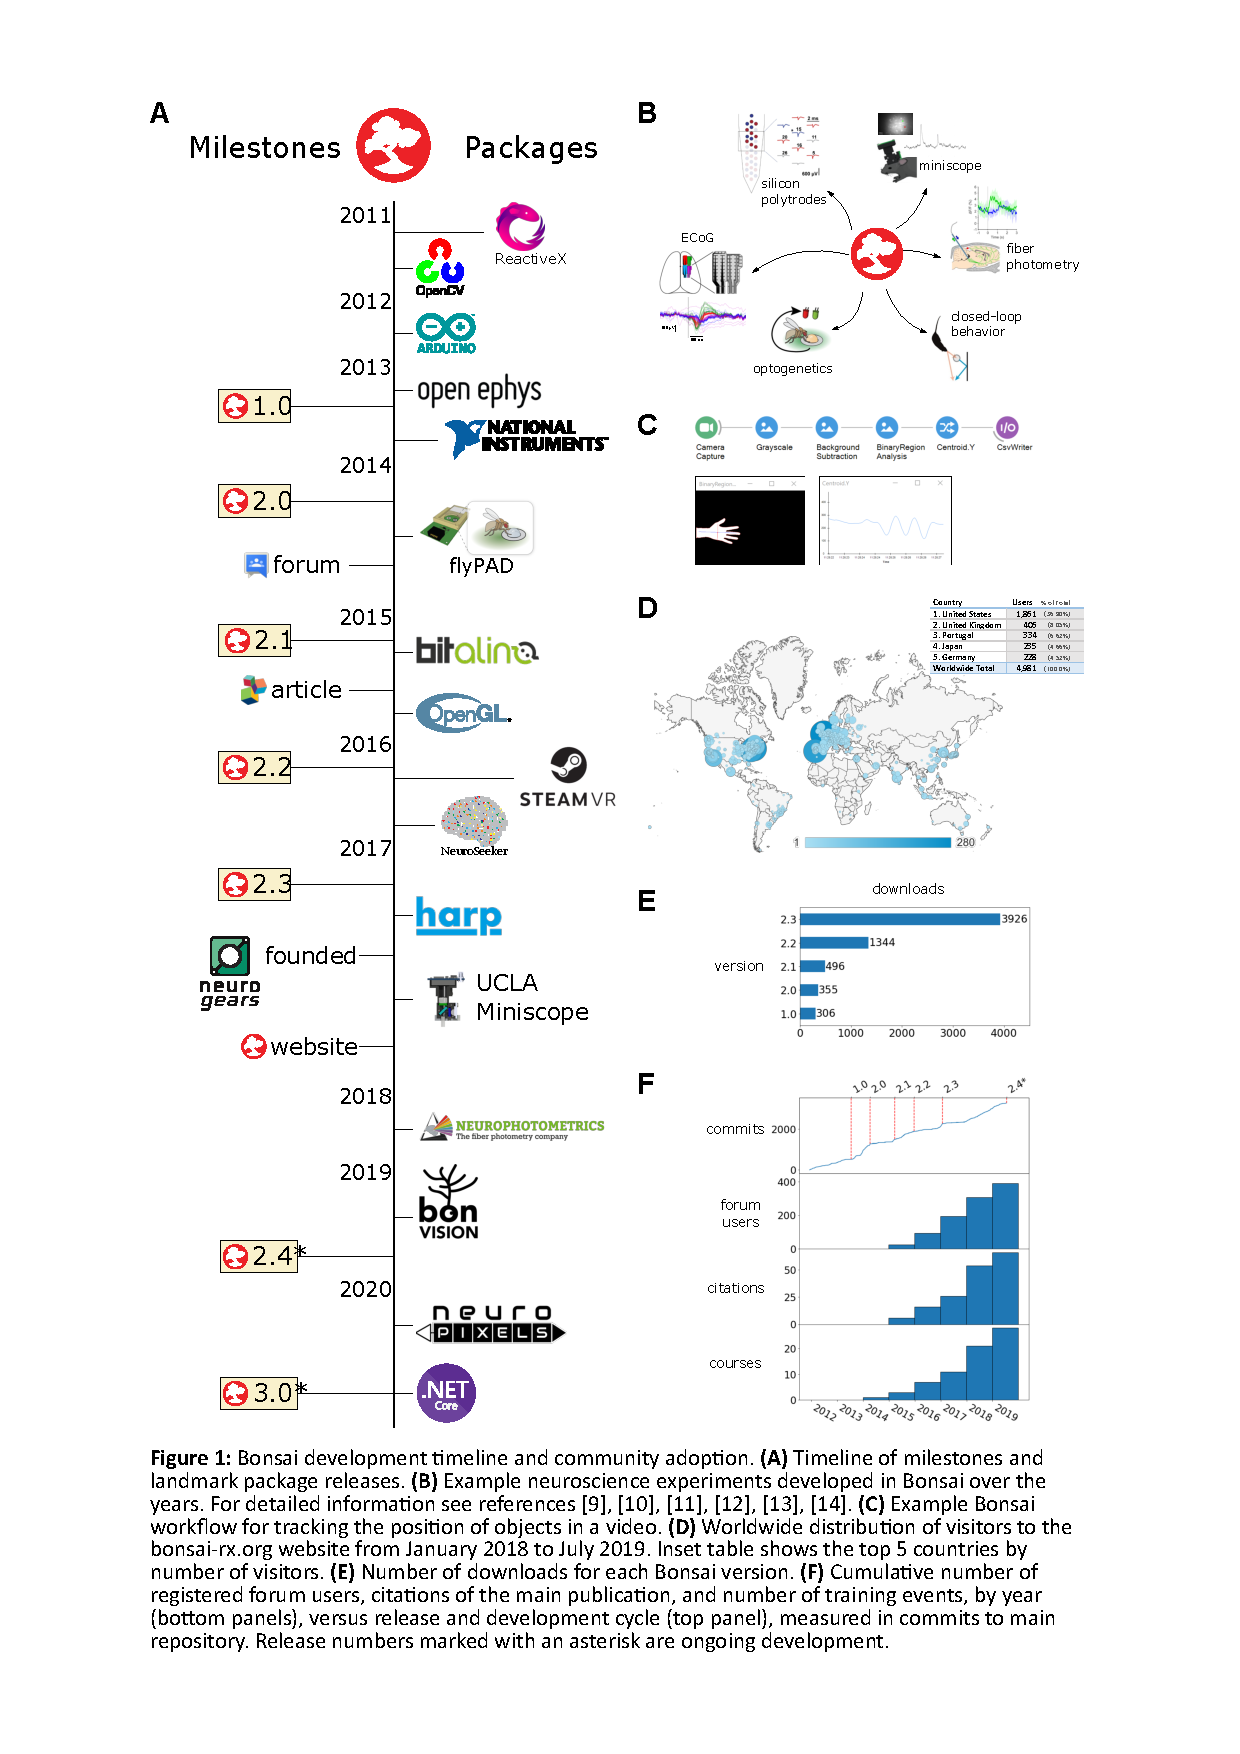
\includegraphics[width=7in]{figures/bonsai.pdf}
        \label{fig:bonsai}
    \end{center}
\end{figure}

\setcounter{figure}{1}

\begin{figure}
    \begin{center}
        
\includegraphics[width=4in]{figures/proposed_bonsai_extensions.png}
        \caption{Proposed extensions to Bonsai}
        \label{fig:proposedBonsaiExtensions}
    \end{center}
\end{figure}

Currently Bonsai has its own package manager, and its community of users have
already extended Bonsai's functionality with several contributed packages
(e.g., \ldots \textcolor{red}{Goncalo please reference the best contributed
packages developed by the Bonsai community}). However, these packages need to
be written in C\#, while most current neuroscience data analysis methods are
written in Python, R or Matlab.  We propose to add to Bonsai capabilities to
communicate with software written in these languages
(Section~\ref{sec:bonsaiPythonMatlabCommunication}).  These capabilities will
allow a large number of neuroscience data analysis methods to be easily
integrated into the Bonsai ecosystem and will provide Bonsai users a large
repertoire of advance machine learning methods for their behavioral and neural
data analysis.

Bonsai is an excellent tool for reproducible data acquisition and
experimental control. An experiment implemented in Bonsai can be replicated in
a new laboratory by just sharing a Bonsai configuration file. With the addition
of the proposed machine learning functionality Bonsai will extend this
reproducibility to the domain of data analysis
(Section~\ref{sec:reproducibility}).

\subsubsection{Bonsai}
\label{sec:bonsai}

Bonsai~\citep{lopesEtAl15,lopesAndMonteiro21} is a free and open-source visual
programming language that emphasizes performance, flexibility, and ease-of-use,
allowing scientists with no previous programming experience to quickly develop
their own high-performance data acquisition and experimental control systems
(Figure 1c). Bonsai combines a high-level event algebra for data streams with
an integrated development environment (IDE) and a strong library of plugins
supporting multiple hardware and software packages used by the biomedical
research community (Figures 1a, 1b).

Bonsai has a large user base in the systems neuroscience community.
Quantifications of this user base are provided in Figures 1d-1f.  In the last
year alone, we estimate more than 1,000 new users have started to incorporate
Bonsai into their experimental protocols across the world. The surprising rate
of adoption of Bonsai in non-programmer experimental labs highlights the need
for accessible programming tools that enable state-of-the-art technology but
also allow researchers to stay in control and change their experimental
paradigms.  Many open-source software tools are either inaccessible to
non-programmers, or too constrained to be of general use outside their narrow
domain of application. Bonsai has been successful because it has straddled this
gap to some extent.

The language has also helped to potentiate the growing wave of foundational
open hardware initiatives, such as the OpenEphys \citep{siegleEtAl17} and UCLA
Miniscope~\citep{caiEtAl16}, making it possible to quickly combine and
integrate these tools into new experiments~\citep{buccinoEtAl18}.
%
Bonsai has been adopted in large neuroscience undertakings like the
International Brain
Laboratory\footnote{\href{https://www.internationalbrainlab.com/}{https://www.internationalbrainlab.com/}}
and the Allen Institute for Brain
Science\footnote{\href{https://alleninstitute.org/what-we-do/brain-science/}{https://alleninstitute.org/what-we-do/brain-science/}}.
%
More recently, Bonsai has started to expand outside the domain of neuroscience
into biomedical research and biotechnology tool development, and even outside
academia into public outreach and education programs.

\subsection{Details of Resource}

\ii The case for support should outline the full details of the resource and 
associated work packages presented in the proposal.

\iitem Indication whether the project proposed to develop a new
resource or is in support of an existing one.

Existing if general Bonsai enhancements.  If specific to analysis we
may be able to argue for "new" if helpful, while still making
reference to Bonsai installed base.  

\iitem Objectives for the proposal should be detailed including
individual measurable targets against which the outcome of the work
will be assessed. This should refer to the objectives set out in the
Je-S proposal form.

\iitem{Significant technical details for the development, maintenance or 
enhancement of the resource must be clearly outlined and indicated 
how this is of internationally exceptional quality. }

\iitem{If applicable, outline any proposed research efforts and how they 
  directly facilitate development of the resource. }

\iitem{For proposals looking to focus on maintaining status quo for an 
existing resource instead of suggesting further development, you 
should detail evidence of why significant upgrades are not required at 
this time and detail why the resource needs continued support to 
maintain world-leading functionality.}

\ii{Additional questions that may be considered: }

\iitem Does the facility begin or continue to support a growing field of 
bioscience, what is the anticipated growth and does the proposal 
adequately accommodate this? 

\iitem How will the resource accelerate science within its field and
  beyond?

\iitem What would be the impact on the scientific community if the resource 
did not exist? How would this impact other, possibly dependent 
resources?

\subsubsection{Video-based behavioral analysis}
\label{sec:videoBasedBehavioralAnalysis}

Precisely quantifying animal behavior is an essential step toward understanding
brain function.  Deeplabcut is a Python-based software for tracking animal body
parts \citep{mathisEtAl18}, which it is currently well integrated with
Bonsai~\citep{kaneEtAl20}. Here we propose extensions to Bonsai to extract
other informative features from video recordings.

\begin{description}

    \item[Motion sequencing]\citep[MoSeq;][]{wiltschkoEtAl15}: extracts patterns
        of behavior that repeat over time (i.e., syllables of behavior) from
        video data. For instance, it parses (in an unsupervised way) the
        behavior of a mouse in an arena into segments of time where a mouse
        was running, rearing and grooming. It uses a hidden Markov model and it
        is implemented in Python\footnote{Code for MoSeq can be requested from
        the Datta laboratory, as indicated at
        \href{http://datta.hms.harvard.edu/research/behavioral-analysis/}{http://datta.hms.harvard.edu/research/behavioral-analysis/}.}.
        After trained MoSeq can be used to detect behavioral syllables online.

    \item[Decoding behavior from neural
        activity]\citep[BehaveNet;][]{battyEtAl19} combines hidden Markov
        models with convolutional autoencoders and discriminative models to
        decode video data from neural recordings. It is implemented in
        Python\footnote{\href{https://github.com/themattinthehatt/behavenet}{https://github.com/themattinthehatt/behavenet}}.
        After trained it can be used online to decode video data and detect
        behavioral syllables.

    \item[Interpretable latents for behavioral videos]\citep[Partitioned
        Subspace Variational Autoencoder, PS-VAE;][]{whitewayEtAl21}: produces
        interpretable low-dimensional representations of behavioral videos by
        combining the output of pose-estimation algorithms (e.g., DeepLabCut)
        with unsupervised dimensionality reduction methods. These
        low-dimensional representations facilitate downstream behavioral and
        neural analyses. It is based on autoencoders and is implemented in
        Python\footnote{code for PS-VAE is embedded in the BehaveNet code
        \href{https://github.com/themattinthehatt/behavenet}{https://github.com/themattinthehatt/behavenet}.
        Please refer to class \texttt{PSVAE} in 
        \texttt{behavenet.models.vaes.py}.}. After trained it can be used
        online to extract low-dimensional features and perform downstream
        processing.

\end{description}

\subsubsection{Spike sorting}
\label{sec:spikeSorting}

\noindent\textcolor{red}{TODO}

\subsubsection{Low-dimensional representations of spiking data}
\label{sec:lowDimensionalRepresentationsOfSpikingData}

Bonsai is well integrated with OpenEphys~\citep{siegleEtAl17}, which allows
scientists to record neural data from a large number of devices. However, it
lacks functionality to process these recordings. Here we describe software that
we propose to integrate into Bonsai to extract interpretable summary statistics
(i.e., latent variables) from neural spiking activity.

\begin{description}

    \item[Gaussian Linear Dynamical
        System]\citep[GLDS;][]{andersonAndMoore12}: with sufficiently large
        bin sizes, spike counts can be modeled as Gaussian random processes.
        This Gaussianity assumption greatly simplifies the estimation of
        parameters of linear dynamical system (LDS) models, as well as
        inferences about their states. After models parameters have been
        learned, GLDS can be used online. A unique feature of GLDS is that the
        posterior distribution of states given all observation up to the
        present can be calculated efficiently. This estimate of the posterior
        distribution can be used online for experimental control, as we
        propose in Section~\ref{sec:comparisonOfMultipleMethods}. We will use an R implementation of GLDS
        which allows the use of external
        inputs\footnote{\href{https://github.com/joacorapela/kalmanFilter}{https://github.com/joacorapela/kalmanFilter}}.

    \item[Poisson Linear Dynamical System]\citep[PLDS;][]{mackeEtAl15}: for
        smaller bin sizes, spike counts are better modeled as Poisson random
        processes, rather than Gaussian ones. The algorithm described in
        \citet{mackeEtAl15} can estimate the parameters of a LDS, and make
        inferences about its states, from Poisson distributed observations.  We
        propose to interface Bonsai with a Matlab implementation of
        PLDS\footnote{\href{https://bitbucket.org/mackelab/pop\_spike\_dyn/src/master/}{https://bitbucket.org/mackelab/pop\_spike\_dyn/src/master/}}
        that uses variational inference. PLDS does not provide online estimates
        of the states, since data from a full trial is needed for state
        inference.

    \item[Hidden Markov Model]\citep[HMM;][]{rabiner89}: as LDSs, HMMs model a
        time series of observations as random processes conditioned on hidden
        states. However, in HMMs hidden states are discrete random variables,
        while in LDSs they are continuous ones. In some application domains
        (e.g., speech, epilepsy) discrete state assumptions are more pertinent
        than continuous ones. We propose to use an R implementation of
        HMMs\footnote{\href{https://github.com/joacorapela/hiddenMarkovModels}{https://github.com/joacorapela/hiddenMarkovModels}}.
        As GLDSs, once trained, HMMs can be used online to infer the posterior
        distribution of states given observations.

    \item[Gaussian Processes Factor Analysis]\citep[GPFA;][]{yuEtAl09}: as
        LDSs, GFPA models represent a time series of observation as random
        processes conditioned on hidden states. However, in GPFA models the
        state dynamics are nonlinear, while in LDS models they are linear.
        Thus, GPFA models are more general than LDS ones. As GLDS models, GPFA
        models assume that observations conditioned on states are Gaussian
        random processes. We propose to use a Matlab implementation of
        GPFA\footnote{\href{https://users.ece.cmu.edu/~byronyu/software/gpfa0203.tgz}{https://users.ece.cmu.edu/~byronyu/software/gpfa0203.tgz}}.
        GPFA models do not provide online estimates of the states, since data
        from the full trial are needed for state estimates.

    \item[Sparse Variational Gaussian Processes Factor
        Analysis]\citep[svGPFA;][]{dunckerAndSahani18}: is similar to GPFA, but
        models point process observations (i.e., single spikes as opposed to
        spike counts). We propose to use a Python implementation of
        svGPFA\footnote{\href{https://github.com/joacorapela/svGPFA}{https://github.com/joacorapela/svGPFA}}.
        svGPFA models do not provide online estimates of states, since data
        from the full trial are needed for state estimates.

    \item[Latent factor analysis through dynamical
        systems]\citep[LFADS;][]{pandarinathEtAl18}: uses an autoencoder
        framework, with recursive neural networks, to infer continuous states
        conditioned on spike counts, similar to those inferred by GPFA. We
        propose to use a Python implementation at
        LFADS\footnote{\href{https://github.com/tensorflow/models/tree/master/research/lfads}{https://github.com/tensorflow/models/tree/master/research/lfads}.}.
        As GPFA, LFADS do not provide online estimates of states.

\end{description}

\subsubsection{Low-dimensional representations of local-field potentials}
\label{sec:lowDimensionalRepresentationsOfLFPs}

Spikes are extracted from a higher-frequency range of extracellulary recorded
voltages. Local field potentials (LFPs) are computed from a lower-frequency
range and are another important signal to understand brain function. We propose
to use states inferred from LFPs by GLDS, GPFA, HMM and LFADS
(Section~\ref{sec:lowDimensionalRepresentationsOfSpikingData}) as
low-dimensional representations of the LFP.

\subsubsection{Neural decoding}
\label{sec:neuralDecoding}

In order to use low-dimensional representations of spiking activity and/or of
LFPs to guide the control of experiments, we need a decoder to optimally map
these low-dimensional representations to experimental controls.
%
We propose to implement in Bonsai several decoding/classification algorithms:
k-nearest neighbor, linear discriminative analysis, support vector machines,
random forests, artificial neural networks, naive Bayes and Gaussian process
classifiers.

\subsubsection{Comparing multiple data-analysis methods}
\label{sec:comparisonOfMultipleMethods}

We propose to add functionality to Bonsai to facilitate multi-method
comparisons in user-supplied datasets. Below we describe a comparison that we
will perform in Bonsai to asses the relative performance of the methods
described in the previous sections with neural recordings from behaving rats.
These recordings are currently being performed, to address scientific questions,
at the laboratory of Prof.~Akrami in the SWC.
%
Details of the experimental task appear in~\citet{akramiEtAl18}.
%
Briefly, in this task there are three nose ports (left, center, right). Rats
initiate a trial by inserting their nose in the center port for the duration of
the fixation period, until they hear a Go stimulus. During the fixation period
two stimuli $s_a$ and $s_b$ are presented. Rats should decide which stimuli is
louder. If $s_a$ is louder than $s_b$ the correct action is to poke the nose
into the right port in order to collect a liquid reward, and if $s_b$ is louder
than $s_a$ the correct choice is the left port.

We will use high-density Neuropixel spike and LFP recordings from the rats
performing this task to learn low-dimensional representations of spiking
activity and LFPs during the decision time period (between the presentation of
the last auditory stimuli and the presentation of the Go stimulus), using the
methods described in
Sections~\ref{sec:lowDimensionalRepresentationsOfSpikingData}
and~\ref{sec:lowDimensionalRepresentationsOfLFPs}. We will also learn the
parameters of the classifiers described in Section~\ref{sec:neuralDecoding} to
optimally classify animal decisions (poke the nose into the right/left port)
based on the previous low-dimensional representations.

We will compare the decoding accuracy of all decoders. This comparison will
tells us, for the auditory working memory task, which neural data type (spikes
or LFPs), which low-dimensional representation method (e.g., LDS or Gaussian
processes), and which decoder (e.g., Bayesian or ANN) yields the best decodings
in state-of-the-art neural recordings from behaving animals.

\subsubsection{Interfacing Bonsai with Python, R and Matlab data analysis software}
\label{sec:bonsaiPythonMatlabCommunication}

Bonsai is written in C\# and most neural data-analysis methods are written in
Python, R or Matlab. Fortunately, there exist software that allow C\# program
to call and be called by programs in these other languages. For the
communication of C\# programs with Python we will use
Python.NET\footnote{\href{https://github.com/pythonnet/pythonnet}{https://github.com/pythonnet/pythonnet}},
with R programs we will use
R.Net\footnote{\href{https://github.com/rdotnet/rdotnet}{https://github.com/rdotnet/rdotnet}}
and with Matlab we will use the built in Matlab .NET
interface\footnote{\href{https://uk.mathworks.com/help/matlab/matlab\_external/using-net-from-matlab-an-overview.html}{https://uk.mathworks.com/help/matlab/matlab\_external/using-net-from-matlab-an-overview.html}}.
In cases where these software cannot support some type of communication between
C\# and another language we will use the messaging library
ZeroMQ\footnote{\href{https://zeromq.org/}{https://zeromq.org/}}.

\subsubsection{Reproducibility with Bonsai}
\label{sec:reproducibility}

The current version of Bonsai facilitates reproducibility of data acquisition
and experimental control across laboratories. Most data acquisition and
experimental control aspects of an experiment can be reproduced across
different laboratories by sharing a Bonsai configuration file.
%
By adding data analysis functionality to Bonsai, besides reproducing my data
acquisition and experimental control, Bonsai users will also be able to reproduce
data analysis functionality.

We will demonstrate each machine intelligence functionality added to Bonsai
(Section~\ref{sec:toBeAddedMachineIntelligenceFunctionality}) and the multiple
data-analysis methods comparisons
(Section~\ref{sec:comparisonOfMultipleMethods}) in Bonsai experiments. We will
then distribute Bonsai configuration files for users to reproduce these
demonstrations.

\subsubsection{Final remarks}
\label{sec:finalRemarks}

We proposed to add machine intelligence functionality to Bonsai to assist users
in building close-loop neural experiments: online spike sorting, methods for
low-dimensional representation of spiking activity and LFPs, and neural
decoding algorithms. This functionality will allow neuroscience Bonsai users to
build more sophisticated experiments and extract more information from their
experimental recordings.

We also proposed to add functionality to help Bonsai users compare the
performance of multiple methods on their datasets. With this functionality
Bonsai users will be able to select the best methods to model their own
recordings. It will also motivate methods developers to interface their
data-analysis functionality with Bonsai. By doing so, they will provide their
software to the large community of Bonsai users, and will be able to easily
compare the performance of their methods with that of preexisting methods in the
Bonsai ecosystem. In this way method developers will become a new type of
Bonsai users, which will guarantee the sustainability of developments
proposed here.

We focused this proposal on neuroscience applications of Bonsai. However, the
addition of machine intelligence functionality is needed in many other
experimental areas where Bonsai is or could be used. Therefore, the software
abstractions that we will build to add to Bonsai machine intelligence
functionality for neuroscience experiments (e.g., methods to perform
multi-method comparisons) will translate to other application domains of
Bonsai.

Multiple groups at the SWC currently use Bonsai for data acquisition and
experimental control. Carefully testing the functionality of new software is
essential to ensure its correct functionality. We propose to use the SWC large
internal Bonsai user base to test the functionality we will add to Bonsai,
before distributing it to the general public.

\subsection{Community Demand}
\ii Evidence of community demand should be primarily driven from UK 
academic researchers working largely within BBSRC remit – see our 
Forward look for UK Bioscience for more detail on research areas covered by 
BBSRC. Demand from other users (such as academic communities outside 
of BBSRC remit or industrial users) may be appropriate to provide additional 
support, especially in highlighting the potential for economic, commercial or 
societal impact, but should not be the focus of the demand demonstration. 
Evidence provided should highlight examples of the high-quality science that 
the resource will underpin or has underpinned. Where possible and relevant, 
examples should be drawn from a wide research community to illustrate the 
broad impact of the resource to support high-quality internationally excellent 
science.  

\ii The level of community demand should be benchmarked against other 
relevant resources and/or the size of the community. This will allow the fair 
assessment of resources with different user bases. The types of evidence 
that may be appropriate to provide will be different for new and existing 
resources. 

\ii Evidence of wider consultation of the prospective community (e.g community 
surveys) is encouraged. 

\iibf New Resources

\ii New resources should estimate the number of researchers who may engage and benefit from the resource. Evidence, where possible, would be of benefit and may include: 
\begin{itemize}
    \item  Datasets (or samples) in public or private repositories 
    \item Citations or acknowledgments 
    \item Gap analysis with existing resources 
    \item Pilot project uptake or feedback from potential users.  
\end{itemize}

\ii In particular, proposals for new resources should have consulted their prospective community prior to application

\iibf Existing Resources

\ii For existing resources this should include usage data of the
current resource. Data types may include: 

\iitem Access requests from independent users/ sites 

\iitem Citations or acknowledgements 

\iitem Other public resources providing links to the resource 

\iitem New major acquisitions captured by the resource 

\ii{Additionally, existing resources need 
to evidence why this resource needs 
to be maintained/updated by the 
current grant. This could include: }

\iitem Survey data from users on what upgrades are needed 

\iitem Evidence of an expanding 
user base, which requires 
additional resource 

\iitem Recent developments in the 
field, which require upgrades 
to be integrated into the 
resource. 


\subsection{User engagement}
\ii Discussion of user engagement provision should aim to answer the following 
questions:

\iitem Is there awareness of the resource within the user community?

\iitem How do you plan to develop the engagement strategy within the 
proposal timeframe to expand user engagement? 

\iitem How have access mechanisms to ensure usability of the resource 
been considered? 

\iitem How have user needs been incorporated into this proposal to ensure 
it is fit for purpose and will deliver on expectations? 

\iibf New Resources
  
\ii Evidence should be provided as to how the resource plans to engage
stakeholders and ensure that the resource meets their needs and is
used by the community targeted by the resource.

\iibf Existing Resources

\ii Evidence should be provided as to whether the resource has
achieved the level of engagement it originally anticipated, and
consideration is given how the additional investment would change
this.  

\subsection{Long term sustainability planning}
\ii{
In addition, the case for support should outline considerations for the long-
term sustainability of the resource beyond UKRI-BBSRC funding, as well as 
the true cost of running and maintaining the resource in question. 
The proposal should include: }

\iitem Cost recovery plans, where appropriate, or an explanation why
not if not viable. Evidence of clear business planning with a focus on
at least partial cost recovery is required, especially when applying
as an existing resource.

\iitem Details for alternative support plans, aside from UKRI-BBSRC 
funding. 

\iitem The level of support the resource is projected to require for expected 
maintenance and/or subsequent maturation/enhancement activities. 
Clear arguments as to why UKRI-BBSRC should support the resource now 
should be provided, if other cost recovery and support plans are deemed 
unsuitable.  


\subsection{Potential for economic and societal impact}
\ii{Outline how the outputs of the proposed resource will contribute to 
knowledge and how this may have the potential for economic return or 
societal benefits. Impact activities should be integrated into appropriate 
sections of the case for support, not presented as an independent work 
package. }

\iitem All proposals are expected to demonstrate clear plans with recorded 
milestones and timelines for associated activities to develop 
economic, commercial and societal impacts.  
August 2021 7 
 

\iitem Methods of engagement and measures of success should be outlined 
including how these will be regularly reviewed throughout the project 
in order to deliver the most impact. 

\iitem Any planned activities should be fully justified within the Justification 
of Resources attachment








\subsection{Track Record}
\ii{
The majority of the track record relevant to the project should be located 
within the Narrative CV and should not be repeated within the case for 
support. You may, however, want to describe: }

\iitem Track record of the team working together  

\iitem Specific expertise available at the host organisation and any 
proposed partner organisations to enable the successful delivery of 
the project.  

\iitem The specific role of each applicant and collaborator in the project


\bibliographystyle{apalike}
\bibliography{bonsai,epsrcSoftwareForResearchCommunities,monitoringBehavior,stateSpaceModels,machineLearning,gaussianProcesses}

\end{document}
